%!TEX root = Report.tex
\chapter{Theory}\label{sec:methodofattack}

\section{Model Building}
In order to measure the local heat coefficient $\alpha$ a valid experimental model is required. To create a model which performs similar to the real heat exchange inside a blade non-dimensional characteristic numbers have to match. Although a turbine blade is internally cooled with air and the presented model uses water, a matching Reynolds number $Re=\frac{\rho v L}{\mu}$ yields in equitable flow conditions. However also Prandtl number $Pr=\frac{\nu}{\alpha}$ and Nusselt number $Nu=\frac{\alpha L}{\lambda}$ have to match in order to guarantee equal thermal conditions and conductivity. Finally another simplification is made by supposing only one-dimensional heat transfer to be relevant.
\begin{figure}[H]
\centering
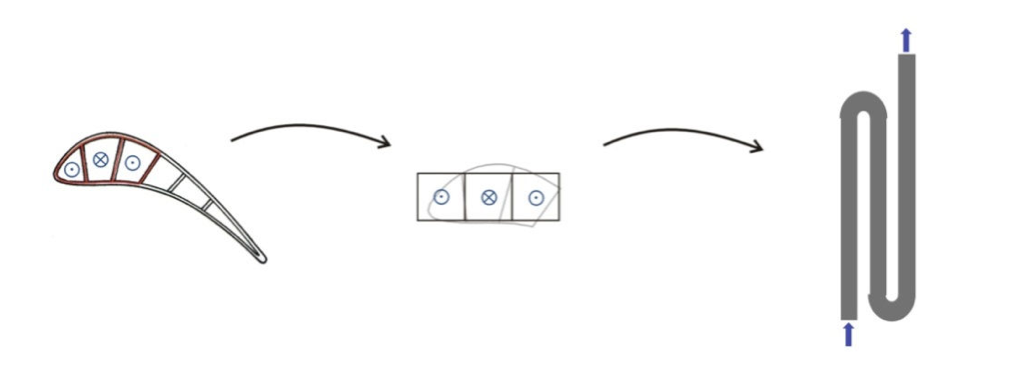
\includegraphics[width=.8\textwidth]{pics/modelbuilding}
\caption{From Blade to Experimental Model}
\label{pic:modelbuilding}
\end{figure}

\section{Heat transfer}

The heat transfer coefficient $\alpha$ is determined from the unsteady one-dimensional heat conduction equation. The assumption for one-dimensional heat transfer is valid, because we consider only a very short time period and because we have only the thickness of the Aluminium plate as relevant geometric parameter, the other dimensions are in comparison very large. The time constant is given in equation \ref{eq:timeconstant}

\begin{equation}
t_{max}=\frac{L^2}{a}=0.9983\ s
\label{eq:timeconstant}
\end{equation}

with a the thermal diffusity defined in equation \ref{eq:diffusity} and $L=10\ mm$. 

\begin{equation}
a=\frac{\lambda}{\rho c_p}=0.10016 \cdot 10^{-3}\ m^2/s
\label{eq:diffusity}
\end{equation} 

where for Aluminium $\lambda=238\ W/mK$, $\rho=2700\ kg/m^3$ and $c_p=880\ J/kg K$. \\

The basic one-dimensional conduction equation is shown in equation \ref{eq:heat1D}.

\begin{equation}
\frac{\partial T}{\partial t}=a \frac{\partial^2 T}{\partial x^2} 
\label{eq:heat1D}
\end{equation}

To solve this equation, we need to specify initial and boundary conditions as given in the following:

\begin{equation}
T(x,t=0) = T_i \nonumber
\end{equation}

\begin{equation}
T(x \rightarrow \infty,t) = T_i \nonumber
\end{equation}

\begin{equation}
\lambda \left. \frac{\partial T}{\partial x}  \right|_{x=0}=\alpha(T_{\infty}-T(0,t)) \nonumber
\end{equation}

where $T_i=51^{\circ}$ is the initial temperature and $T_{\infty}=10^{\circ}$ the fluid temperature.

The solution of the differential equation is evaluated at $ T(x=0,t)=T_s $ and can be seen in equation \ref{eq:sol}. 

\begin{equation}
\frac{T_s-T_i}{T_{\infty}-T_i}=1-\exp \left( \frac{\alpha^2 a t}{\lambda^2}\right)  \operatorname{erfc} \left( \frac{\alpha \sqrt{a t}}{\lambda} \right)
\label{eq:sol}
\end{equation}

In the measurement, we obtain the surface temerature in function of the time. As we want to determine $\alpha$, we have to solve this equation but it is not linear in $\alpha$ and can not be solved explicitely. Therfore the delivered MATLAB file calculates the solution numerically.


\section{Thermochromic Liquid Crystals (TLC)}

With the help of Thermochromic Liquid Crystals (TLC), the surface temperature is visualized. TLC react to change of temperatures by changing their colors. This substance shows properties between a crystalline solid and an isotropic liquid. \\

The long chain organic molecules are aligned in a certain direction. In order to reach a dense packing, the molecules are arranged with a slight twist. On a larger scale, this leads to a helical orientation. This helix has a pitch (distance over which  molecule rotates over $360^\circ$). Light hitting this structure is transmitted and reflected. Only the component of the light which has circular polarization with the same hand sign as the helix direction is transmitted, while all others are reflected. In consequence, when white light hits the structure, only one particular wavelength is reflected.\\

As the temperature changes, the helical structure varies. Increasing the temperature leads to two effects: thermal expansion of the helice which increases pitch and faster twist which decreases twist. The second effect is usually dominating. This results in a diminution of the molecule and a color change to shorter wavelengths.\\

In our experiment we use TLC with a temperature range from $35^\circ$C to $37^\circ$C. When the temperature is out of this range, the crystals appear black. Before the actual experiment, a calibration has to be done to allocate the different colorings to a particular temperature, which has been already done for us.



